%-------------------------------------------------------------------------------
%-------------------------------------------------------------------------------
%-------------------------------------------------------------------------------
\chapter{Méthode de Newton}
%-------------------------------------------------------------------------------
%-------------------------------------------------------------------------------
\thispagestyle{empty}

%--------------------------------------------------------------------------
%--------------------------------------------------------------------------
\section{L'algorithme}
%-------------------------------------------------------------------------------
%-------------------------------------------------------------------------------
On rappelle l'algorithme associé à la méthode de Newton

%--------------------------------------------------------------------------
\begin{lstlisting}
def Newton(f, f_prime, a, epsilon):
    """ Entrées : deux fonctions réelles, 2 réels
        Requis : f est C1 sur un intervalle contenant a
                 f_prime est la dérivée de f
                 epsilon > 0
        Sortie : c appartenant à [a;b] tel qu'il existe un 
                 zero c' de f avec |c - c'| de l'ordre de epsilon """
    x = a
    ecart = 1 + epsilon
    while ecart >= epsilon:
        x_old = x
        x = x - f(x)/f_prime(x)
        ecart = abs(x - x_old)
    return x
\end{lstlisting}
%--------------------------------------------------------------------------
%--------------------------------------------------------------------------
Pour visualiser le comportement de cet algorithme, on souhaite suivre les évolutions des valeurs calculées. On remplace alors le critère d'approximation ($\varepsilon$) par un critère de nombre d'itérations.
%--------------------------------------------------------------------------
%--------------------------------------------------------------------------
\begin{Exercise}\it
Écrire une fonction \type{suite\_Newton(f, df, x0, n)} renvoyant la liste des  valeurs de la suite $(x_k)$ définie par la méthode de Newton appliquée à $f$, de premier terme $x_0$, pour $0 \le k \le n$.
\end{Exercise}
%--------------------------------------------------------------------------
\begin{Answer}
\begin{lstlisting}
def suite_Newton(f, df, x0, n):
    X = [0]*(n+1)
    X[0] = x0
    for i in range(n):
        x = X[i]
        X[i+1] = x - f(x)/df(x)
    return X
\end{lstlisting}
\end{Answer}
%--------------------------------------------------------------------------
%--------------------------------------------------------------------------
\section{Un exemple}
%-------------------------------------------------------------------------------
%-------------------------------------------------------------------------------
On considère le polynôme $P=X^4+X^3-23X^2+3X+90$

\begin{figure}[h!]
   \centering
   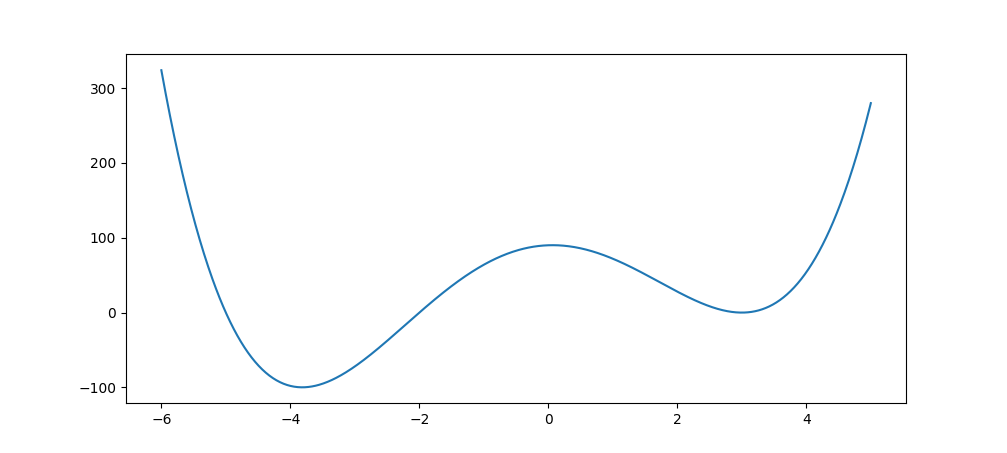
\includegraphics[scale=0.6]{TP/Images/20_poly.png}
   \caption{\label{polyn} Graphe du polynôme $P$}
\end{figure}
%--------------------------------------------------------------------------
%--------------------------------------------------------------------------
\begin{Exercise}\it
Créer les fonctions \type{P(x)} et \type{dP(x)} qui calculent respectivement la valeur de $P(x)$ et de $P'(x)$.
\end{Exercise}
%--------------------------------------------------------------------------
\begin{Answer}
\begin{lstlisting}
def P(x):
 return 90 + x*(3 + x*(-23+x*(1+x)))
 
def dP(x):
 return 3 + x*(-46+x*(3+x*4))
\end{lstlisting}
\end{Answer}
%--------------------------------------------------------------------------
%--------------------------------------------------------------------------
\medskip

On va rechercher des racines de $P$ en utilisant la méthode de Newton. 

%--------------------------------------------------------------------------
\begin{Exercise}\it
Déterminer les suites de valeurs fournies par \type{suite\_Newton(p, dP, x0, 10)} avec $x_0$ prenant les valeurs dans $\{ -10, -8, -6, -4, -2, 0, 2, 4\}$. 

Tracer sur un seul graphe les lignes formées des points $(k,x_k)$ pour chaque valeur initiale.

Quelles semblent être les racines de $P$ ?

\end{Exercise}
%--------------------------------------------------------------------------
\begin{Answer}
\begin{lstlisting}
for x0 in [-10, -8, -6, -4, -2, 0, 2, 4]:
    X = suite_Newton(P, dP, x0, 10)
    plt.plot(X)
plt.show()
\end{lstlisting}
\begin{center}
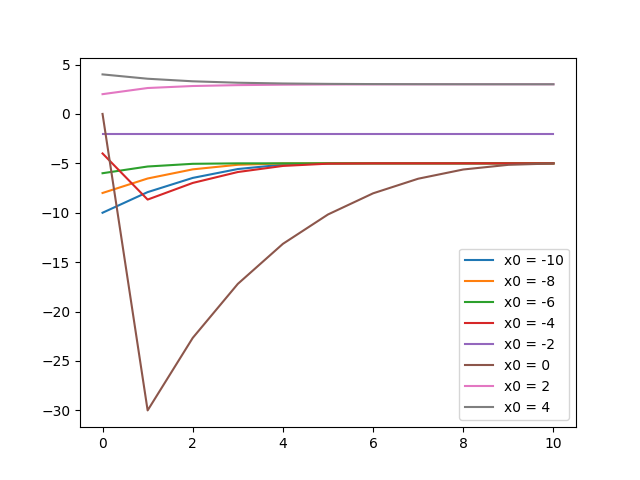
\includegraphics[scale=0.9]{20_Newtons}
\end{center}
\end{Answer}
%--------------------------------------------------------------------------
%--------------------------------------------------------------------------
\section{Sensibilité aux conditions initiales}
%--------------------------------------------------------------------------
%--------------------------------------------------------------------------
Dans les calculs précédents on a vu que les zéros calculés pouvaient s'entremêler : 
les conditions initiales $-4$, $-2$ et 0 donnaient respectivement $-5$, $-2$ et $0$ comme valeur de racines de $P$. Nous allons explorer ce genre de phénomène.
%--------------------------------------------------------------------------
%--------------------------------------------------------------------------
\begin{Exercise}\it
Écrire une fonction \type{suite(a, b, n)} qui renvoie une liste de $n$ valeurs régulièrement espacées entre $a$ et $b$.
\end{Exercise}
%--------------------------------------------------------------------------
\begin{Answer}
\begin{lstlisting}
def suite(a, b, n):
    pas  = (b-a)/(n-1)
    X = [0]*n
    for i in range(n):
        X[i] = a + pas*i
    return X
\end{lstlisting}
\end{Answer}
%--------------------------------------------------------------------------
%--------------------------------------------------------------------------
\begin{Exercise}\it
Après avoir déterminé \type{X = suite(-5, 2, 100000)} calculer la liste \type{Y} telle que 
\type{Y[i]} est le zéro renvoyé par \type{Newton(p, dP, X[i], 0.00001)} et tracer le graphe correspondant (\type{plt.plot(X, Y)}).
\end{Exercise}
%--------------------------------------------------------------------------
\begin{Answer}
\begin{lstlisting}
X = suite(-5, 2, 100000)
Y = [Newton(P, dP, x, 0.0001)[0] for x in X]
plt.plot(X, Y)
plt.show()
\end{lstlisting}
\begin{center}
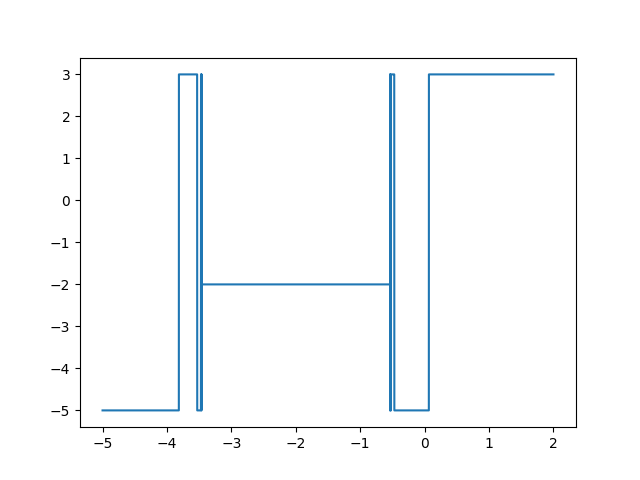
\includegraphics[scale=0.9]{20_limites}
\end{center}
\begin{lstlisting}
a = -0.5361498906
n = 8
for k in range(n):
    h = 10**(-k)
    X = suite(a-h, a+h, 10000)
    Y = [Newton(P, dP, x, 0.0001) for x in X]
    plt.subplot((n+1)//2, 2, k+1)
    plt.plot(X, Y)
plt.show()
\end{lstlisting}
\begin{center}
\hbox{}\kern -3cm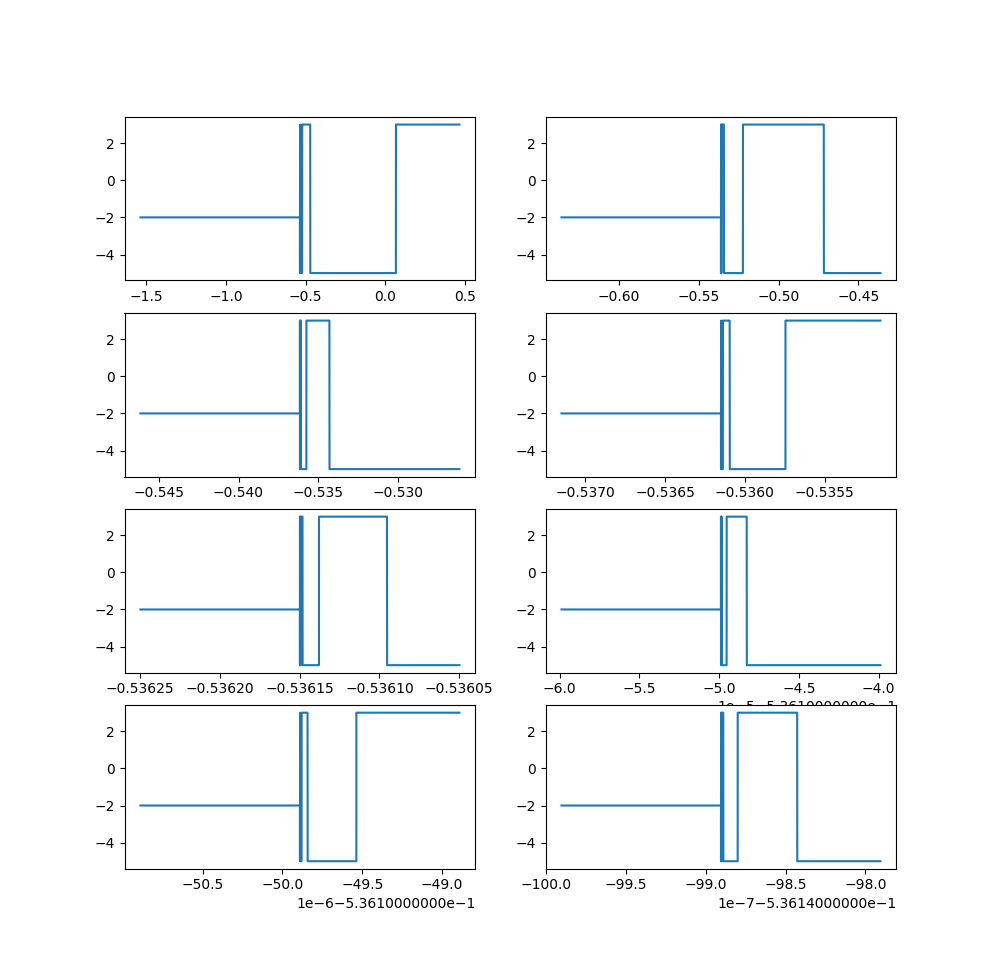
\includegraphics[scale=0.7]{20_fractals}
\end{center}
\end{Answer}
%--------------------------------------------------------------------------
%--------------------------------------------------------------------------
Si on agrandit le graphe autour de $x = -0.5361498906$ on voit apparaître un comportement fractal : le même motif apparaît à plusieurs échelles.
%--------------------------------------------------------------------------
\newpage
%--------------------------------------------------------------------------
\section{Sans la dérivée}
%--------------------------------------------------------------------------
%--------------------------------------------------------------------------
Il est parfois difficile de connaître la dérivée d'une fonction.

\begin{itemize}
    \item Dans ce cas on peut utiliser la méthode de dichotomie, mais elle est moins efficace que la méthode de Newton.

\item On peut aussi utiliser, dans la méthode de Newton, la droite passant par $\bigl(x, f(x)\bigr)$ et $\bigl(x_{old}, f(x_{old})\bigr)$ (la sécante) à la place de la dérivée. $x$ et $x_{old}$ sont les deux derniers points calculés par la méthode.

On voit qu'on a besoin de deux points initiaux pour démarrer l'algorithme.

L'équation de la sécante est $\displaystyle Y = f(x) +\frac{X - x}{x_{old} - x}\bigl(f(x_{old}) - f(x)\bigr)$ donc le point d'intersection de la sécante 
avec l'axe des abscisses est $(x', 0)$ avec $\displaystyle x' = x - \frac{f(x)(x - x_{old})}{f(x) - f(x_{old})}$.
%--------------------------------------------------------------------------
%--------------------------------------------------------------------------
\begin{Exercise}[title = Méthode de la sécante]\it
Écrire une fonction  \type{secante(f, a, b, epsilon)} retournant une valeur approchée à $\varepsilon$ près d'une racine $r$ de $f$ en utilisant la méthode de la sécante ; $a$ et $b$ sont les deux valeurs utilisées pour la première sécante.
\end{Exercise}
%--------------------------------------------------------------------------
\begin{Answer}
\begin{lstlisting}
def secante(f, a, b, epsilon):
    x_old = a
    x = b
    while abs(x - x_old) >= epsilon:
        x_new = x - f(x)*(x -x_old)/(f(x) - f(x_old))
        x_old = x
        x = x_new
    return x
\end{lstlisting}
\end{Answer}
%--------------------------------------------------------------------------
%--------------------------------------------------------------------------
\item Une autre modification de la méthode de Newton est de remplacer le calcul de la dérivée par une valeur approchée.

On choisit l'approximation symétrique  : $\displaystyle f'(x) \sim \frac{f(x+h) - f(x-h)}{2h}$.
%--------------------------------------------------------------------------
%--------------------------------------------------------------------------
\begin{Exercise}\it
Écrire une fonction  \type{der(f, x, h)} qui renvoie une valeur approchée de $f'(x)$ par cette méthode.
\end{Exercise}
%--------------------------------------------------------------------------
\begin{Answer}
\begin{lstlisting}
def der(f, x, h):
    return (f(x+h) - f(x-h))/(2*h)
\end{lstlisting}
\end{Answer}
%--------------------------------------------------------------------------
%--------------------------------------------------------------------------
\begin{Exercise}[title = Méthode de la pseudo-dérivée]\it
Écrire une fonction  \type{Newton1(f, a, epsilon)} retournant une valeur approchée à $\varepsilon$ près d'une racine $r$ de $f$ en utilisant la méthode ci-dessus. On pourra choisir $h = \frac{\varepsilon}{10}$.
\end{Exercise}
%--------------------------------------------------------------------------
\begin{Answer}
\begin{lstlisting}
def Newton1(f, a, epsilon):
    h = epsilon/10
    x = a
    ecart = 1 + epsilon
    while ecart >= epsilon:
        x_old = x
        x = x - f(x)/der(f, x, h)
        ecart = abs(x - x_old)
    return x
\end{lstlisting}
\end{Answer}
%--------------------------------------------------------------------------
%--------------------------------------------------------------------------
\item On peut surtout utiliser une fonction de la  bibliothèque numérique : \type{fsolve} se trouve dans la sous-bibliothèque \type{scipy.optimize}.

C'est la méthode à privilégier dans les calculs scientifiques.
%--------------------------------------------------------------------------
%--------------------------------------------------------------------------
\begin{Exercise}Lire la documentation de \type{fsolve}.

Comment calculer un zéro de $x \mapsto a^x - x^2-2$ en fonction du paramètre $a$ ?

\end{Exercise}
%--------------------------------------------------------------------------
\begin{Answer}
\begin{lstlisting}
from scipy.optimize import fsolve

def f(x, a):
    return a**x - x**2 - 2
    
z = fsolve(f, 3, args = (2))
\end{lstlisting}
\end{Answer}
%--------------------------------------------------------------------------
%--------------------------------------------------------------------------

\end{itemize}